\chapter{Design} % (fold)
\label{cha:design}

\section{Software Architecture} % (fold)
\label{sec:software_architecture}
\subsection{Relationship with Cocoa Touch Framework} % (fold)
\label{sub:relationship_with_cocoa}

Core Data, Core Location, WebKit, MapKit, UIKit are used in this project. As shown in Figure~\ref{fig:relationships},  NSManagedObject, NSObject, UITableViewController, UIViewController are inherited by different classes.
\label{sec:data_model}
\begin{figure}
	\centering
    \SetFigLayout{1}{1}
    {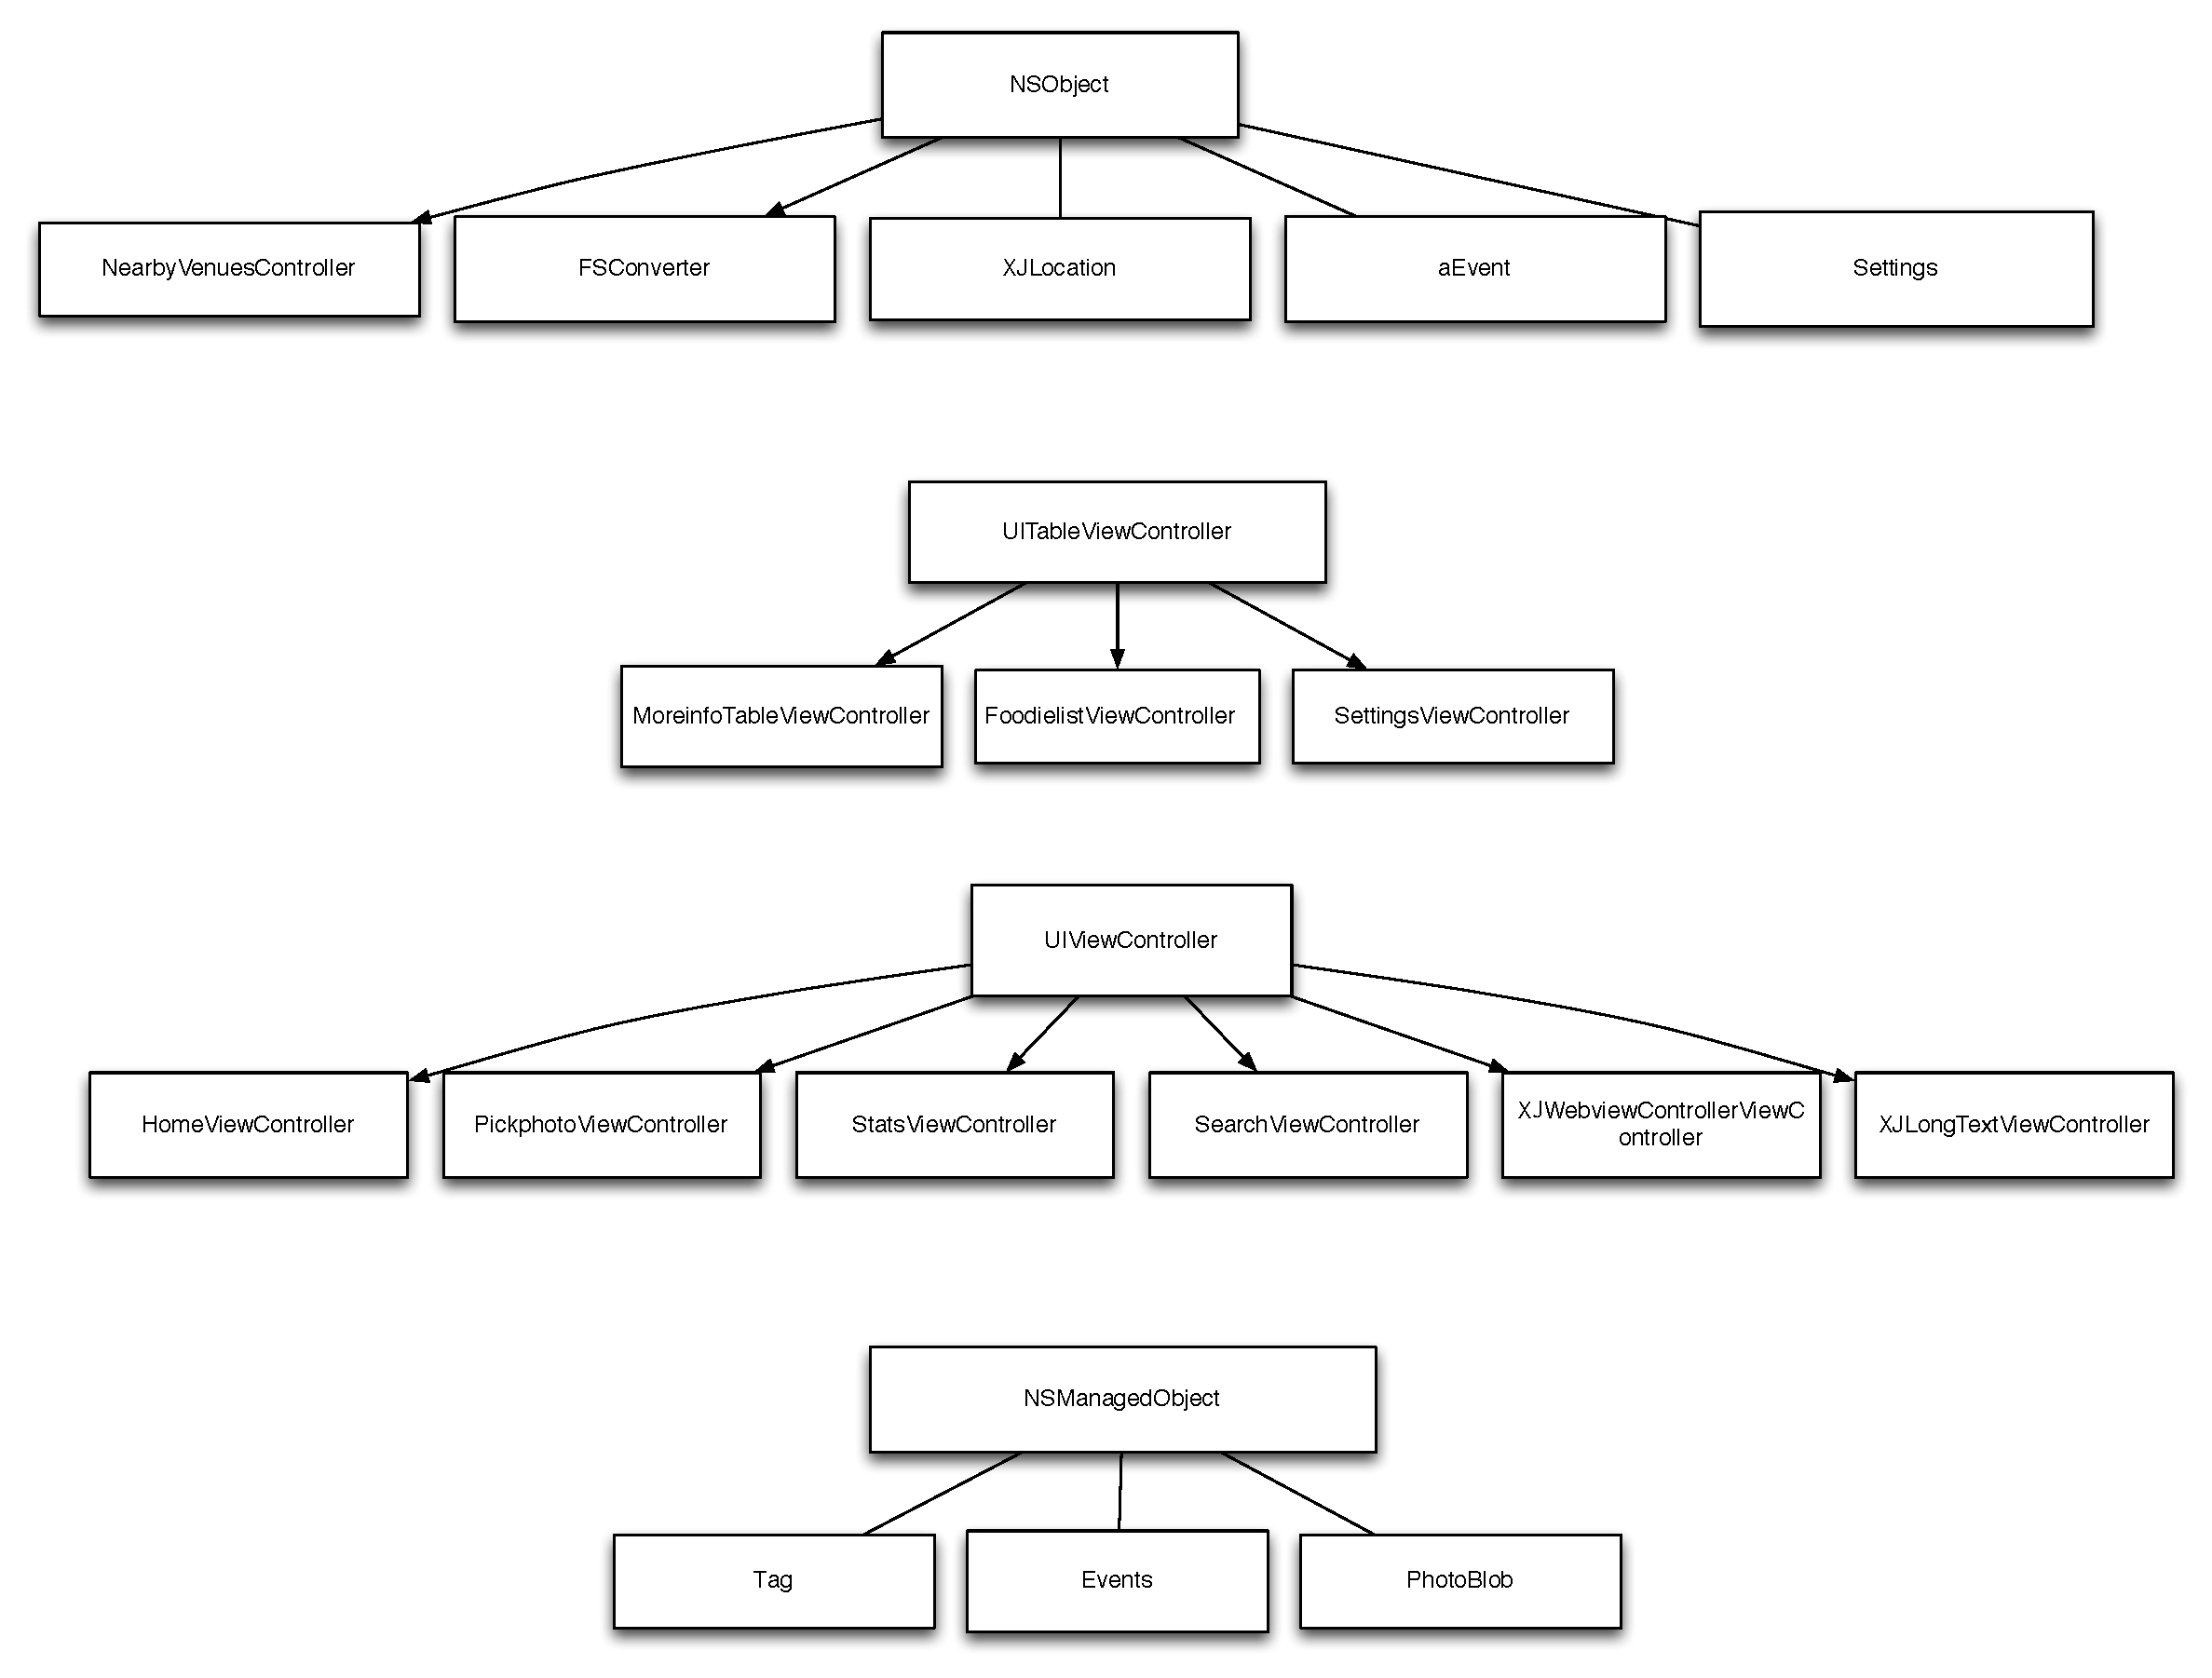
\includegraphics[%
    width=\figwidth, totalheight=\figheight, keepaspectratio]{./relationships.pdf}}
    \caption{Relationships with Cocoa Touch Framework}
	\label{fig:relationships}
\end{figure}
% subsection relationship_with_cocoa (end)
\subsection{Database Schema} % (fold)
\label{sub:database_schema}

	We used three tables for storing all the information from user. As Figure~\ref{fig:data-schema} shows, Events is the main table in the app. It provides fields ``address'', ``comment'', ``creationDate'', ``latitude'', ``longitude'', ``locationName'', ``rate'', ``thumbnail'', ``photoBlob'' and ``tags''. ``address'' field is used when user didn't find their ``locationName'' in location list which fetched from Foursquare API v2. ``Latitude'' and ``longitude'' is used for adding annotations in Map View. A 80*80 resolution thumbnail is stored for each event in order to accelerate loading food list table. \\ 
	
	``photoBlob'' has one to one relationship with ``photo'' in PhotoBlob table. Using a separate table should also help speeding up when we don't need to load photo while we still need to get the meta data of the event. \\
	
	Field ``tags'' has many to many relationship with ``photos'' in Tag table because one photo can labeled with many tags and one tag can relate to many photos.  
	

\begin{figure}
	\centering
    \SetFigLayout{1}{1}
    {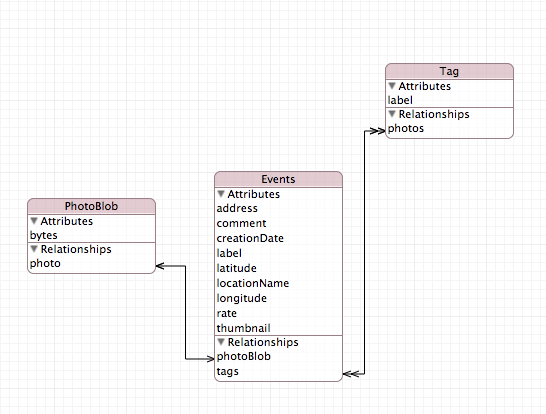
\includegraphics[%
    width=\figwidth, totalheight=\figheight, keepaspectratio]{./screenshots/database_schema.png}}
    \caption{Database Schema}
	\label{fig:data-schema}
\end{figure}

% subsection database_schema (end)

\subsection{Settings Property List} % (fold)
\label{sub:settings_list}

	When developing under iOS, we can also use another way to store the data we need. \emph{Property List} is used to store all information related to the app itself. For instance, using \emph{Property List} to store app display name, app version are commonly used in all apps for iPhone. \\
	
	``Fancy Foodie'' uses release number as main version string and git hash tag of the release as build string, so ``1.0 (build 3df55bb)'' is shown in Figure~\ref{fig:settings} which means that the main version number is 1.0 and build hash tag is 3df55bb. \\
	 
	 This app also use \emph{Property List} to store whether we need to save photo to album locally. If this option is enabled, the app will create an album  named ``Fancy Foodie Photos'' and put photos when creating the event in this album as shown in Figure~\ref{fig:album}.
% subsection settings_list (end)
% section software_architecture (end)



\section{Modules} % (fold)
\label{sec:modules}
Figure~\ref{fig:classdiagram} shows all the classes and public methods in the project. 

\begin{figure}
	\centering
    \SetFigLayout{1}{1}
    {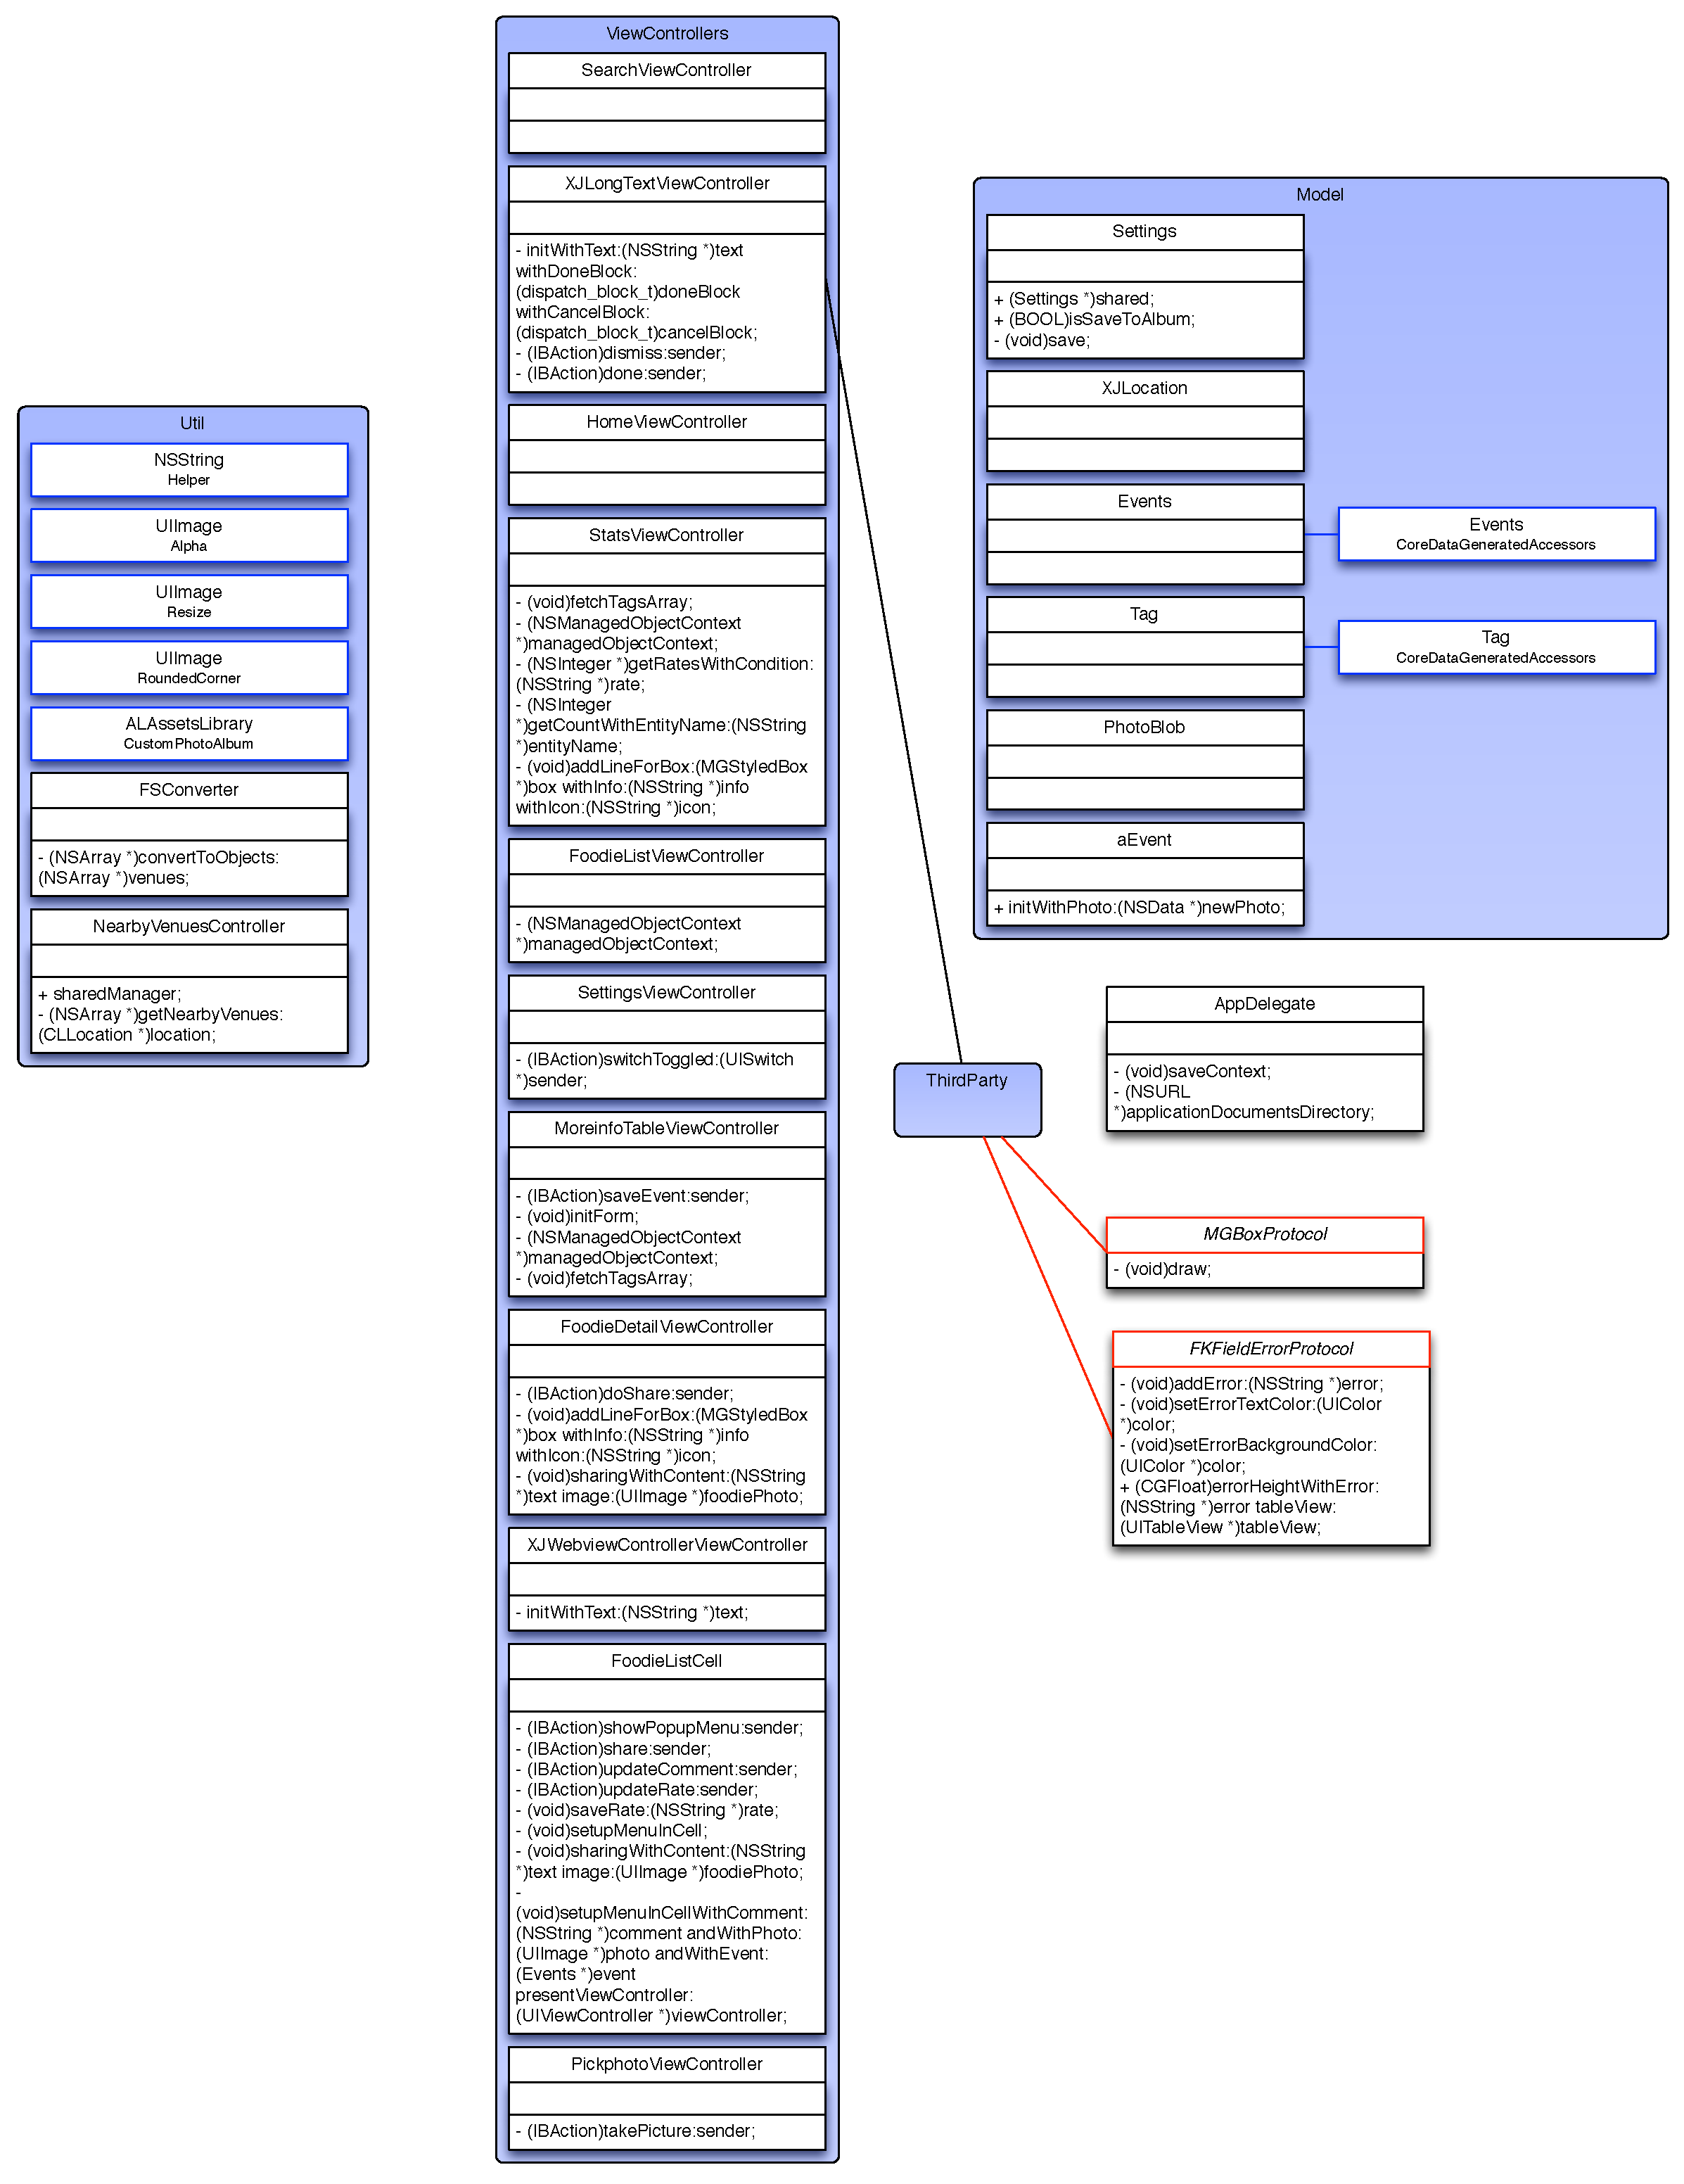
\includegraphics[%
    width=\figwidth, totalheight=\figheight, keepaspectratio]{./UML_Fancy.pdf}}
    \caption{Class-diagram of the project}
	\label{fig:classdiagram}
\end{figure}
% subsection overview_of_modules (end)

\subsection{View Controllers} % (fold)
\label{sub:view_controllers}
	Figure~\ref{fig:storyboard} shows main views in storyboard. In this project, we build it as a tab based application. Five tabs are created for different purposes. Home tab plays as a guide to create a food event; Food list tab shows all the events created before; Statistics tab shows all aggregated data; Searching tab is used to show all past events and searching by address to find the events; Setting tab is for configurations.
	
\begin{figure}
	\centering
    \SetFigLayout[5]{1}{1}
    {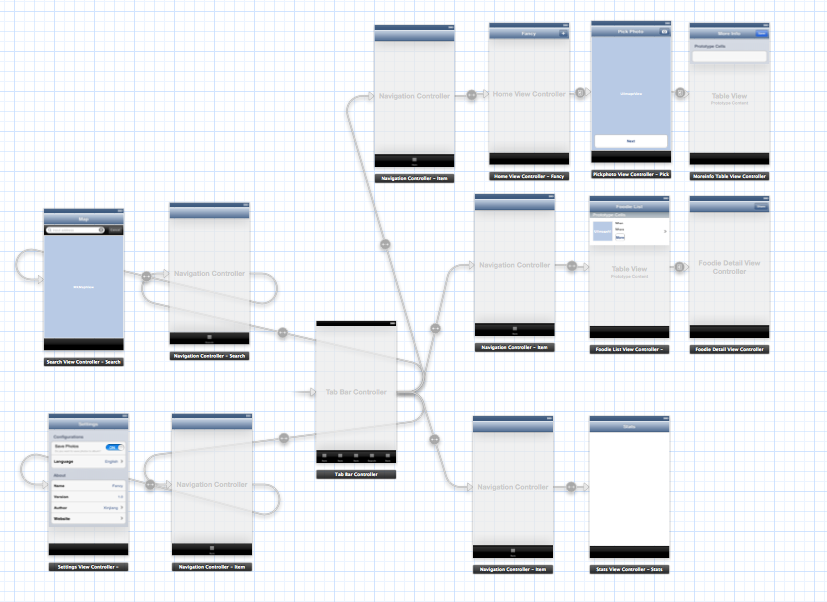
\includegraphics[%
    width=\figwidth, totalheight=\figheight, keepaspectratio]{./screenshots/storyboard-full.png}}
    \caption{Storyboard of Overview Fancy Foodie}
	\label{fig:storyboard}
\end{figure}

	The correspond viewControllers are list as follows.
	 
\begin{description}
	\item[HomeViewController] \ \hfill 
	Control views for users to start using the app.
	\item[PickphotoViewController] \ \hfill
	Present a preview of the photo chosen.
	\item[MoreinfoTableViewController] \ \hfill
	Control a form with all different types of information need to create a event.
	\item[FoodieListViewController] \ \hfill
	Display a table view to show all food events with thumbnail, relative date and location info. Control the logic of updating comments and rates.
	\item[XJLongTextViewController] \ \hfill
	Embedded a UITextView in UIViewController.
	\item[FoodieDetailViewController] \ \hfill
	Display all information of a particular event.
	\item[StatsViewController] \ \hfill
	Show statistics of all events.
	\item[SearchViewController] \ \hfill
	Provide a MKMapView, UISearchDisplayController and UITableView in this controller. 
	\item[SettingsViewController] \ \hfill
	Setting Options such as ``Save photo'',``language''. App name, version, author and support website are controlled here as well.
	\item[XJWebviewControllerViewController] \ \hfill
	Provide a UIViewController embedded with UIWebView.
\end{description}
% subsection view_controllers (end)

% subsection models (end)

\subsection{Third Party Libraries and Utility} % (fold)
\label{sub:third_party_and_utilities}
The following is a list of third party libraries used in the project.
		\begin{itemize}
		    \item TestFightSDK: Beta Testing on the fly.
		    \item BaseKit: Tools to create singleton class and better Location Manager.
			\item QBPopupMenu: Pop-up Menu User Interface
			\item CZPhotoPickerController: Preview of photos and better photo picker.
			\item FormKit: Form style tableview creation.
			\item BButton: Button with twitter bootstrap color schema.
			\item Foursquare2: Foursquare API version 2.
			\item MGBox: Table style boxes creation.
			\item SORelativeDateTranformer: Convert date to relative date such as ``One day ago''.
			\item FontAwesome: Adding icons to user interface.
			\item SVProgressHUD: Notification messages display.
		 \end{itemize}
A few important utility classes are listed as follows. 
		\begin{itemize}
		    \item NearbyVenuesController: Making request to Foursquare to get a list of locations nearby.
		    \item UIImage(Resize), UIImage(Alpha), UIImage(RoundedCorner): Tools to resize and modify images.
			\item ALAssetsLibrary(CustomPhotoAlbum): Saving images to custom album.
			\item FSConverter: Converting Foursquare feedback to an object.
			\item NSString(Helper): Providing convenient methods of NSString. 
		 \end{itemize}

% subsection third_party_and_utilities (end)
% section modules (end)

\section{Key Methods} % (fold)
\label{sec:main_methods}

\subsection{Insert New Event} % (fold)
\label{sub:insert_new_event}
	Figure~\ref{fig:storyboard-home} shows the procedure to add a new event. - (IBAction)saveEvent:(id)sender; in class MoreinfoTableViewController is called when a user finished editing all information in the form. First of all, we checked whether the save photo option is on or not. If it is on, we should save the image to an album named ``Fancy Foodie Photos''. Otherwise, go ahead and create an instance of Events called newEvent. Afterward, we assign all the information from user interface and save. Next step is to use the navigationController to pop to root view controller which is HomeViewController.

\begin{figure}
	\centering
    \SetFigLayout{1}{1}
    {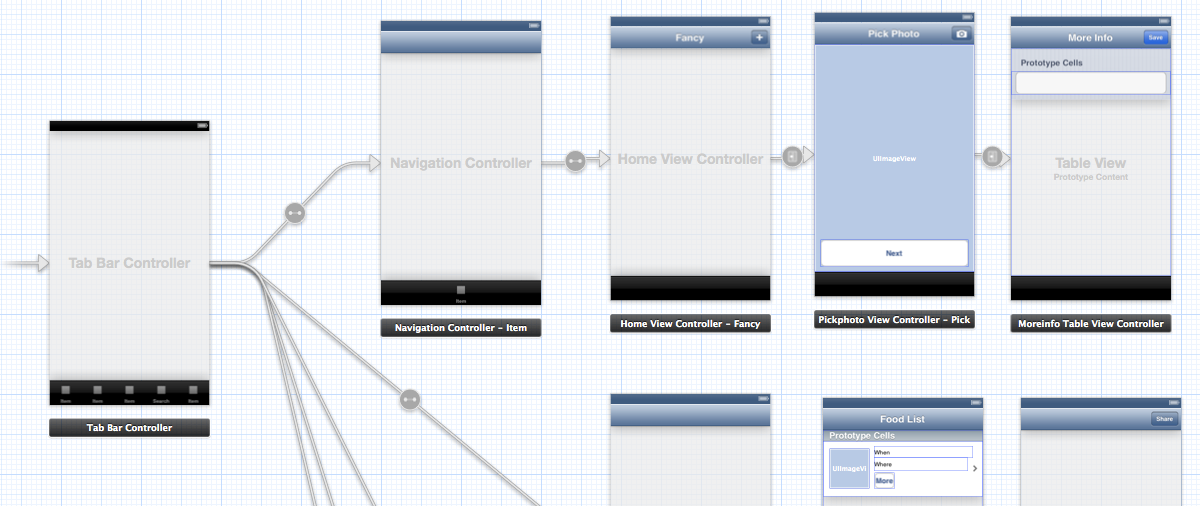
\includegraphics[%
    width=\figwidth, totalheight=\figheight, keepaspectratio]{./screenshots/storyboard-home.png}}
    \caption{Storyboard of Home Tab View}
	\label{fig:storyboard-home}
\end{figure}
% subsection insert_new_event (end)

\subsection{Update Event} % (fold)
\label{sub:update_event}

Updating event is actually updating rate or comment. When a user tapped on the pop up menu and chose comment option in Figure~\ref{fig:foodlist-menu}, - (IBAction)updateComment:(id)sender; in class FoodieListCell is called. Class XJLongTextViewController is used and presented as a modal (Figure~\ref{fig:foodlist-comment}). After typing in new comment and done button is tapped , it uses  NSManagedObjectContext to save the event and stored the updated data in the local database.

\begin{figure}
	\centering
    \SetFigLayout{1}{1}
    {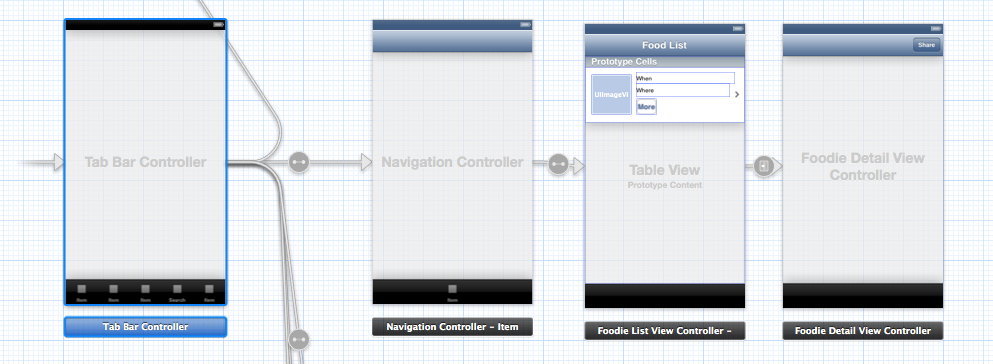
\includegraphics[%
    width=\figwidth, totalheight=\figheight, keepaspectratio]{./screenshots/storyboard-foodlist.png}}
    \caption{Storyboard of Food List Tab View}
	\label{fig:storyboard-foodlist}
\end{figure}

% subsection update_event (end)

\subsection{Delete Event} % (fold)
\label{sub:delete_event}

	Delete event is very simple in this app. In food list tab, you'll see a list of events. Swiping from right to left enable the delete button as shown in Figure~\ref{fig:foodlist-delete}.  After tapping on the button, - (void)tableView:(UITableView *)tableView commitEditingStyle:(UITableViewCellEditingStyle)editingStyle forRowAtIndexPath:(NSIndexPath *)indexPath; in class FoodieListViewController is called. In the method, it uses NSManagedObjectContext deleteObject to delete the event and save the result in local database after save function is called. Afterward, current tableview is refreshed as well.
% subsection delete_event (end)

\subsection{Searching Events} % (fold)
\label{sub:searching_logic}
	
	Searching events is done with MapKit API. All the events are fetched in during loading time. The events are annotated with red pins when the tab is loaded.   \\
	As shown in Figure~\ref{fig:map-address}, as the user is typing in the address, the searching string is passed to -(BOOL)searchDisplayController:(UISearchDisplayController *)controller
shouldReloadTableForSearchString:(NSString *)searchString; , so in that function, we're using CLGeocoder to guess the possible locations for that string. The possible locations are displayed in a table view. After the use choose one possible location, the central region will be focused on that area. At this time, the nearby events stored in database will appear in front of the user.
	

% section main_methods (end)
% chapter design (end)